\documentclass[11pt,a4paper,spanish]{book}
\usepackage{estilo_unir-1}
\usepackage{float}
\hypersetup{
	colorlinks   = true, %Colours links instead of ugly boxes
	urlcolor     = blue, %Colour for external hyperlinks
	linkcolor    = black, %Colour of internal links
	citecolor   = red %Colour of citations
}
\usepackage[nottoc]{tocbibind}

%---------------------------
%título de la asignatura, trabajo y autor
%---------------------------

\subject{Álgebra Lineal en Computación Cuántica}
\title{Producto tensorial y Esfera de Bloch}
\author{Enrique Prada Vázquez}
\profesor{Francisco Costa Cano}
\date{08-05-2026}

\begin{document}
\renewcommand{\listfigurename}{Índice de figuras}
\renewcommand{\listtablename}{Índice de tablas}
\renewcommand{\contentsname}{Índice de contenidos}
\renewcommand{\figurename}{Figura}
\renewcommand{\tablename}{Tabla} 

\maketitle
\frontmatter
\tableofcontents
\listoffigures
\listoftables

\chapter*{Resumen}

En este Trabajo se aborda de forma sistemática la manipulación de sistemas cuánticos multiqubit, fundamentando el análisis en el uso del producto tensorial y en la interpretación geométrica de los estados mediante la esfera de Bloch. A lo largo de la memoria, se presentan los cálculos detallados para la construcción de operadores compuestos a partir de matrices de Pauli, así como la evaluación de amplitudes de transición entre estados específicos de la base computacional. 

El Trabajo integra el desarrollo analítico con la verificación computacional en \textit{Qiskit}, analizando finalmente el comportamiento de las puertas lógicas fundamentales ($X, Y, Z, H$) como rotaciones unitarias en el espacio de estados. Los resultados subrayan la importancia de la fase y la superposición en la evolución de la información cuántica.

\vspace{0.5cm}
\noindent {\bf Palabras clave:} Producto tensorial, esfera de Bloch, operadores unitarios, superposición, matrices de Pauli, Qiskit.

\chapter*{Abstract}

This Report systematically addresses the manipulation of multi-qubit quantum systems, basing the analysis on the use of the tensor product and the geometric interpretation of states through the Bloch sphere. Throughout this document, detailed calculations for the construction of composite operators from Pauli matrices are presented, alongside the evaluation of transition amplitudes between specific computational basis states. 

The Report integrates analytical development with computational verification using \textit{Qiskit}, ultimately analyzing the behavior of fundamental quantum logic gates ($X, Y, Z, H$) as unitary rotations within the state space. The results highlight the significance of phase and superposition in the evolution of quantum information.

\vspace{0.5cm}
\noindent {\bf Keywords:} Tensor product, Bloch sphere, unitary operators, superposition, Pauli matrices, Qiskit.
\mainmatter

\chapter{Introducción}

\section{Motivación y justificación}

El surgimiento del paradigma de la computación cuántica se fundamenta en la necesidad crítica de trascender las limitaciones físicas de la computación clásica \citep{landauer1961}, un desafío que fue anticipado teóricamente por \cite{benioff1980} al describir el primer modelo mecánico-cuántico de un computador. Esta transición se justifica por la ineficiencia intrínseca de los sistemas clásicos para simular la naturaleza a escala atómica; como argumentó \cite{feynman1982}, la simulación de sistemas cuánticos en hardware convencional conlleva un crecimiento exponencial de recursos computacionales, lo que exige el desarrollo de dispositivos que operen bajo las leyes de la superposición y la interferencia \citep{deutsch1985}.

En el escenario tecnológico actual, el diseño de algoritmos cuánticos demanda un dominio absoluto del álgebra lineal y de la manipulación de estados en espacios de Hilbert de alta dimensionalidad. La capacidad de procesamiento de estos sistemas reside en la estructura de sus operadores unitarios y en la explotación del paralelismo cuántico \citep{shor1994}. Por tanto, la comprensión de la construcción de matrices multiqubit y su visualización mediante la esfera de Bloch \citep{bloch1946} no constituye únicamente un ejercicio académico, sino que se establece como una competencia técnica indispensable para el desarrollo de la computación cuántica en la era NISQ \citep{preskill2018}.

\section{Planteamiento del Trabajo}

Este Trabajo se centra en el análisis formal de la composición de sistemas cuánticos a través de la operación del producto tensorial. El problema central reside en la "maldición de la dimensionalidad" que caracteriza a los sistemas de $n$ qubits, donde el espacio de estados escala como $2^n$ \citep{nielsen2010}. El Trabajo aborda este reto mediante el rigor del cálculo analítico de productos de Kronecker y su validación empírica mediante herramientas de computación en la nube.

Se pretende validar la construcción de operadores multiqubit, evaluar su impacto mediante el cálculo de amplitudes de transición y mapear estas operaciones como rotaciones isométricas en el espacio de estados. Se espera que este Trabajo contribuya a consolidar una metodología que integre la precisión del cálculo manual con la eficiencia de las librerías de programación cuántica contemporáneas, garantizando la reproducibilidad de los resultados.

\section{Estructura del Trabajo}

Para alcanzar los objetivos propuestos y resolver de manera sistemática los problemas planteados, este Trabajo se organiza en los siguientes capítulos:

El \textbf{Capítulo 2, Objetivos}, define las metas generales y específicas, estableciendo los umbrales de dominio teórico y práctico requeridos. El \textbf{Capítulo 3, Enunciado del problema}, desglosa los ejercicios prácticos, desde el cálculo de productos de Kronecker en sistemas de cuatro qubits hasta la dinámica de puertas lógicas. 

El \textbf{Capítulo 4, Desarrollo del Trabajo}, constituye el núcleo de la memoria y se articula en tres áreas de análisis. Comienza con el \textbf{cálculo del producto tensorial}, donde se aborda la resolución analítica de los operadores $A, B$ y $C$ para explorar la expansión del espacio de Hilbert. Seguidamente, en el apartado de \textbf{aplicaciones y amplitudes}, se detalla la construcción del operador compuesto $O$ y el cálculo de elementos de matriz fundamentados en la linealidad del producto escalar. Finalmente, el bloque de \textbf{esfera de Bloch y puertas cuánticas} se centra en la representación geométrica de las bases fundamentales y en el análisis rotacional de las puertas $X, Y, Z$ y $H$, bajo el formalismo de evolución unitaria \citep{nielsen2010}.

Finalmente, el \textbf{Capítulo 5, Conclusiones}, sintetiza los hallazgos y evalúa la convergencia entre los resultados analíticos y la simulación realizada en \textit{Qiskit}, seguido de la \textbf{Bibliografía} que recoge las fuentes originales citadas.\begin{itemize}
    \item \textbf{Capítulo 2. Objetivos:} Se definen las metas generales y específicas, estableciendo los niveles de dominio teórico y práctico que se pretenden alcanzar.
    \item \textbf{Capítulo 3. Enunciado del problema:} Se desglosan los ejercicios propuestos, desde el cálculo de productos de Kronecker en sistemas de hasta cuatro qubits hasta la visualización de la dinámica de puertas cuánticas.
    \item El \textbf{Capítulo 4, Desarrollo del Trabajo}, constituye el núcleo de la memoria y se articula en torno a tres áreas clave de análisis. Comienza con el \textbf{cálculo del producto tensorial}, donde se aborda la resolución analítica de los operadores $A, B$ y $C$ con el fin de explorar la expansión del espacio de Hilbert en sistemas multiqubit. Seguidamente, en el apartado de \textbf{aplicaciones y amplitudes}, se detalla la construcción del operador compuesto $O$ y el cálculo minucioso de elementos de matriz fundamentados en la linealidad del producto escalar. Finalmente, el bloque dedicado a la \textbf{esfera de Bloch y puertas cuánticas} se centra en la representación geométrica de las bases fundamentales y en el análisis rotacional de las puertas $X, Y, Z$ y $H$, siguiendo para ello el formalismo de evolución unitaria descrito por \cite{nielsen2010}.
    \item \textbf{Capítulo 5. Conclusiones:} Se sintetizan los hallazgos del Trabajo, evaluando la convergencia entre los resultados analíticos y la simulación computacional realizada con \textit{Qiskit}.
\end{itemize}

Finalmente, se incluye una sección de \textbf{Bibliografía} con las fuentes originales y libros de consulta que han servido de tributo y apoyo documental a las ideas aquí expuestas.

\chapter{Objetivos}

El propósito de este Trabajo es profundizar en el formalismo matricial de la mecánica cuántica, estableciendo un puente entre el cálculo analítico de operadores y su aplicación práctica en entornos de programación cuántica.

\section{Objetivo general}
Desarrollar una comprensión sólida de la estructura algebraica de los sistemas multiqubit y validar su comportamiento mediante la representación geométrica en la esfera de Bloch.

\section{Objetivos específicos}
Para la consecución del objetivo general, se han definido las siguientes metas:

\begin{itemize}
    \item \textbf{Dominio del álgebra de Kronecker:} Dominar la técnica del producto tensorial para expandir operadores de un solo qubit a espacios de Hilbert de mayor dimensión ($2^N$), asegurando la correcta disposición de los elementos matriciales.
    \item \textbf{Análisis de Operadores Compuestos:} Evaluar la acción de operadores complejos definidos por combinaciones lineales de productos de matrices de Pauli, comprendiendo cómo influyen los coeficientes en el elemento de matriz final.
    \item \textbf{Abstracción Geométrica de Puertas:} Caracterizar las puertas cuánticas fundamentales no solo como operadores matemáticos, sino como transformaciones físicas de rotación, facilitando la comprensión de la evolución de estados.
    \item \textbf{Integración Computacional:} Utilizar librerías de computación cuántica (\textit{Qiskit}) para automatizar la construcción de operadores y la visualización de estados, contrastando los resultados numéricos con los desarrollos teóricos.
    \item \textbf{Evaluación de Amplitudes:} Calcular probabilidades y amplitudes de transición entre estados base específicos para determinar la eficacia de las operaciones unitarias aplicadas.
\end{itemize}

\chapter{Enunciado del problema}

El presente Trabajo tiene como objetivo la resolución de una serie de ejercicios prácticos centrados en el álgebra de sistemas cuánticos multiqubit y su interpretación geométrica. El problema se descompone en los siguientes bloques de estudio:

\section{Cálculo de productos tensoriales}
Se requiere determinar la representación matricial resultante de diversas combinaciones de matrices unitarias fundamentales (matrices de Pauli e Identidad), aplicando la operación del producto de Kronecker. En particular, se deben calcular los operadores correspondientes a:
\begin{itemize}
    \item Un sistema de cuatro qubits definido por $A = X \otimes I \otimes Z \otimes I$.
    \item Un sistema de cuatro qubits definido por $B = I \otimes Y \otimes Z \otimes X$.
    \item Un sistema de tres qubits definido por $C = Z \otimes X \otimes I$.
\end{itemize}

\section{Operadores compuestos y amplitudes de transición}
A partir de la combinación lineal de productos tensoriales, se debe definir un operador global $O$ de la forma:
\[ O = \frac{2}{3}(X \otimes Z \otimes I) + \frac{1}{4}(I \otimes Z \otimes X) - \frac{5}{6}(Y \otimes Y \otimes Z) \]
Posteriormente, el problema exige el cálculo de la amplitud de transición (o elemento de matriz) entre dos estados específicos de la base computacional de tres qubits:
\[ \langle 101 | O | 010 \rangle \]

\section{Representación en la esfera de Bloch}
El último bloque del problema se centra en la visualización geométrica mediante el uso de la esfera de Bloch, abordando dos tareas:
\begin{enumerate}
    \item \textbf{Representación de estados:} Localizar en una única esfera los estados cuánticos puros $|0\rangle$, $|1\rangle$, $|+\rangle$, $|-\rangle$, $|i+\rangle$ y $|i-\rangle$.
    \item \textbf{Dinámica de puertas cuánticas:} Visualizar y analizar el efecto de las puertas unitarias $X$, $Y$, $Z$ y $H$ (Hadamard) cuando actúan sobre los estados básicos de la computación $|0\rangle$ y $|1\rangle$.
\end{enumerate}

La resolución de estos puntos debe acompañarse de una implementación práctica en lenguaje Python, utilizando las librerías \texttt{NumPy} para el cálculo matricial y \texttt{Qiskit} para la simulación y visualización de los estados cuánticos.

\chapter{Desarrollo del Trabajo}

\section{Cálculo del producto tensorial}

Para el desarrollo de los ejercicios, se parte de las definiciones de las matrices unitarias de Pauli y la matriz Identidad, las cuales constituyen la base para los operadores de un único qubit:

\[ 
I = \begin{pmatrix} 1 & 0 \\ 0 & 1 \end{pmatrix}, \quad 
X = \begin{pmatrix} 0 & 1 \\ 1 & 0 \end{pmatrix}, \quad 
Y = \begin{pmatrix} 0 & -i \\ i & 0 \end{pmatrix}, \quad 
Z = \begin{pmatrix} 1 & 0 \\ 0 & -1 \end{pmatrix} 
\]

El producto tensorial (o de Kronecker) $A \otimes B$ permite extender estos operadores a espacios de Hilbert de mayor dimensión. Para dos matrices $A$ (de tamaño $m \times n$) y $B$, se define como:
\[ A \otimes B = \begin{pmatrix} a_{11}B & \cdots & a_{1n}B \\ \vdots & \ddots & \vdots \\ a_{m1}B & \cdots & a_{mn}B \end{pmatrix} \]

A continuación, se detallan las combinaciones solicitadas:

\subsection{Caso 1: $X \otimes I \otimes Z \otimes I$}
Este operador actúa sobre un sistema de 4 qubits, resultando en una matriz de $16 \times 16$. Para facilitar su visualización, representamos la matriz resultante en bloques de $8 \times 8$:

\[
X \otimes I \otimes Z \otimes I = 
\begin{pmatrix}
\mathbf{0}_{8 \times 8} & \mathbf{M}_1 \\
\mathbf{M}_1 & \mathbf{0}_{8 \times 8}
\end{pmatrix}
\]

Donde cada bloque $\mathbf{M_1}$ es el producto tensorial de $I \otimes Z \otimes I$, resultando en una matriz diagonal de $8 \times 8$ con la siguiente estructura:

\[
\mathbf{M_1} = I \otimes Z \otimes I = 
\begin{pmatrix}
1 & 0 & 0 & 0 & 0 & 0 & 0 & 0 \\
0 & 1 & 0 & 0 & 0 & 0 & 0 & 0 \\
0 & 0 & -1 & 0 & 0 & 0 & 0 & 0 \\
0 & 0 & 0 & -1 & 0 & 0 & 0 & 0 \\
0 & 0 & 0 & 0 & 1 & 0 & 0 & 0 \\
0 & 0 & 0 & 0 & 0 & 1 & 0 & 0 \\
0 & 0 & 0 & 0 & 0 & 0 & -1 & 0 \\
0 & 0 & 0 & 0 & 0 & 0 & 0 & -1 
\end{pmatrix}
\]

De este modo, la matriz completa de $16 \times 16$ se construye situando el bloque $\mathbf{M_1}$ en las posiciones donde la matriz $X$ tiene sus elementos iguales a 1 (fuera de la diagonal principal) y matrices nulas donde $X$ tiene ceros. Esta estructura es consistente con los resultados obtenidos mediante \texttt{NumPy} en el cuaderno de prácticas.

\subsection{Caso 2: $I \otimes Y \otimes Z \otimes X$}
Este operador actúa sobre un sistema de 4 qubits, lo que genera una matriz de dimensiones $2^4 \times 2^4 = 16 \times 16$. Debido a que el primer qubit se encuentra en el estado Identidad ($I$), la matriz global presenta una estructura diagonal por bloques de $8 \times 8$:

\[
I \otimes Y \otimes Z \otimes X = 
\begin{pmatrix}
\mathbf{M}_2 & \mathbf{0}_{8 \times 8} \\
\mathbf{0}_{8 \times 8} & \mathbf{M}_2
\end{pmatrix}
\]

Para determinar el contenido de los bloques $\mathbf{M_2}$, calculamos primero el producto tensorial de los dos últimos qubits, $Z \otimes X$ (matriz de $4 \times 4$):

\[
Z \otimes X = 
\begin{pmatrix} 1 \cdot X & 0 \cdot X \\ 0 \cdot X & -1 \cdot X \end{pmatrix} =
\begin{pmatrix}
0 & 1 & 0 & 0 \\
1 & 0 & 0 & 0 \\
0 & 0 & 0 & -1 \\
0 & 0 & -1 & 0
\end{pmatrix}
\]

A continuación, aplicamos la matriz $Y = \begin{pmatrix} 0 & -i \\ i & 0 \end{pmatrix}$ sobre el resultado anterior para obtener el bloque $\mathbf{M_2} = Y \otimes (Z \otimes X)$:

\[
\mathbf{M_2} = 
\begin{pmatrix} 
0 \cdot (Z \otimes X) & -i \cdot (Z \otimes X) \\ 
i \cdot (Z \otimes X) & 0 \cdot (Z \otimes X) 
\end{pmatrix} =
\begin{pmatrix}
0 & 0 & 0 & 0 & 0 & -i & 0 & 0 \\
0 & 0 & 0 & 0 & -i & 0 & 0 & 0 \\
0 & 0 & 0 & 0 & 0 & 0 & 0 & i \\
0 & 0 & 0 & 0 & 0 & 0 & i & 0 \\
0 & i & 0 & 0 & 0 & 0 & 0 & 0 \\
i & 0 & 0 & 0 & 0 & 0 & 0 & 0 \\
0 & 0 & 0 & -i & 0 & 0 & 0 & 0 \\
0 & 0 & -i & 0 & 0 & 0 & 0 & 0
\end{pmatrix}
\]

La matriz final de $16 \times 16$ se completa situando dos copias de esta matriz $\mathbf{M_2}$ en la diagonal principal. Es notable observar cómo la presencia de la matriz $Y$ introduce la unidad imaginaria en la estructura, mientras que la matriz $Z$ en la tercera posición del producto tensorial provoca la inversión de fase (cambio de signo de $i$ a $-i$) en los elementos correspondientes a la segunda mitad del bloque $\mathbf{M_2}$. Esta configuración ha sido validada computacionalmente, confirmando el resultado.

\subsection{Caso 3: $Z \otimes X \otimes I$}
Este operador actúa sobre un sistema de 3 qubits, lo que resulta en una matriz de $2^3 \times 2^3 = 8 \times 8$. Utilizando la definición de la matriz $Z$, podemos particionar el operador en dos bloques principales de $4 \times 4$:

\[ 
Z \otimes X \otimes I = \begin{pmatrix} 1 \cdot (X \otimes I) & \mathbf{0} \\ \mathbf{0} & -1 \cdot (X \otimes I) \end{pmatrix} = 
\begin{pmatrix} 
\mathbf{M}_3 & \mathbf{0}_{4 \times 4} \\
\mathbf{0}_{4 \times 4} & -\mathbf{M}_3
\end{pmatrix}
\]

Desarrollando el bloque $\mathbf{M_3} = X \otimes I$:
\[
\mathbf{M_3} = \begin{pmatrix} 0 & 0 & 1 & 0 \\ 0 & 0 & 0 & 1 \\ 1 & 0 & 0 & 0 \\ 0 & 1 & 0 & 0 \end{pmatrix}
\]

Sustituyendo los valores, obtenemos la matriz final expandida:
\[ 
Z \otimes X \otimes I = 
\begin{pmatrix} 
0 & 0 & 1 & 0 & 0 & 0 & 0 & 0 \\
0 & 0 & 0 & 1 & 0 & 0 & 0 & 0 \\
1 & 0 & 0 & 0 & 0 & 0 & 0 & 0 \\
0 & 1 & 0 & 0 & 0 & 0 & 0 & 0 \\
0 & 0 & 0 & 0 & 0 & 0 & -1 & 0 \\
0 & 0 & 0 & 0 & 0 & 0 & 0 & -1 \\
0 & 0 & 0 & 0 & -1 & 0 & 0 & 0 \\
0 & 0 & 0 & 0 & 0 & -1 & 0 & 0 
\end{pmatrix} 
\]
Esta representación muestra claramente cómo el primer qubit ($Z$) controla el signo de los bloques inferiores, mientras que el segundo qubit ($X$) gestiona la posición de los elementos dentro de cada bloque.

\section{Aplicaciones del producto tensorial}

Se define el operador $O$ mediante la suma ponderada de tres términos multiqubit. La construcción de este operador se realiza sumando las contribuciones de cada producto de Kronecker escalado por sus respectivos coeficientes:

\[ O = \frac{2}{3}(X \otimes Z \otimes I) + \frac{1}{4}(I \otimes Z \otimes X) - \frac{5}{6}(Y \otimes Y \otimes Z) \]

La matriz resultante de $8 \times 8$ presenta una estructura simétrica con elementos puramente reales. A continuación, se muestra su representación explícita:

\[
O = \left(
\begin{array}{cccccccc}
0 & 1/4 & 0 & 0 & 2/3 & 0 & 5/6 & 0 \\
1/4 & 0 & 0 & 0 & 0 & 2/3 & 0 & -5/6 \\
0 & 0 & 0 & -1/4 & -5/6 & 0 & -2/3 & 0 \\
0 & 0 & -1/4 & 0 & 0 & 5/6 & 0 & -2/3 \\
2/3 & 0 & -5/6 & 0 & 0 & 1/4 & 0 & 0 \\
0 & 2/3 & 0 & 5/6 & 1/4 & 0 & 0 & 0 \\
5/6 & 0 & -2/3 & 0 & 0 & 0 & 0 & -1/4 \\
0 & -5/6 & 0 & -2/3 & 0 & 0 & -1/4 & 0 
\end{array} \right)
\]

\subsection{Cálculo de la amplitud $\langle 101 | O | 010 \rangle$}
Para hallar este valor, aplicamos la linealidad del producto escalar sobre cada término de $O$:

\begin{enumerate}
    \item \textbf{Término 1:} $\frac{2}{3} \langle 1|X|0\rangle \langle 0|Z|1\rangle \langle 1|I|0\rangle$. Como $\langle 1|I|0\rangle = 0$, este término es nulo.
    \item \textbf{Término 2:} $\frac{1}{4} \langle 1|I|0\rangle \langle 0|Z|1\rangle \langle 1|X|0\rangle$. Como $\langle 1|I|0\rangle = 0$, este término es nulo.
    \item \textbf{Término 3:} $-\frac{5}{6} \langle 1|Y|0\rangle \langle 0|Y|1\rangle \langle 1|Z|0\rangle$. Como $\langle 1|Z|0\rangle = 0$ (ya que $Z|0\rangle = |0\rangle$ y $\langle 1|0\rangle = 0$), este término también es nulo.
\end{enumerate}

Por lo tanto, el resultado final es $\langle 101 | O | 010 \rangle = 0$. Esto demuestra que el estado $|010\rangle$ es ortogonal al estado resultante de aplicar $O$ sobre $|101\rangle$.

\section{Visualización en la esfera de Bloch}

La esfera de Bloch constituye una herramienta fundamental para la representación geométrica de estados puros de un qubit. En la \textbf{Figura \ref{fig:bloch_states}}, se presenta la distribución conjunta de los seis estados solicitados, los cuales se sitúan en los extremos de los ejes ortogonales del espacio de Hilbert:

\begin{itemize}
    \item \textbf{Eje $Z$ (Base computacional):} Los estados $|0\rangle$ y $|1\rangle$ se ubican en los polos norte (rojo) y sur (azul) respectivamente.
    \item \textbf{Eje $X$ (Base de Hadamard):} Los estados $|+\rangle$ y $|-\rangle$ se sitúan en las intersecciones con el eje $X$ ($\theta=\pi/2, \phi=0, \pi$), representados en azul claro y morado.
    \item \textbf{Eje $Y$ (Base circular):} Los estados $|i+\rangle$ y $|i-\rangle$ corresponden a las intersecciones con el eje $Y$ ($\theta=\pi/2, \phi=\pi/2, 3\pi/2$), identificados con los colores verde y amarillo.
\end{itemize}

\begin{figure}[H]
    \centering
    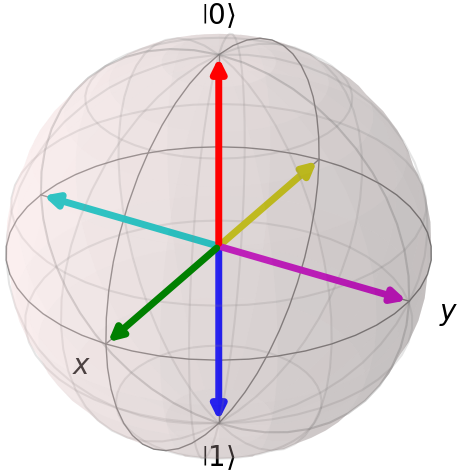
\includegraphics[width=0.55\textwidth]{figuras/esfera_bloch_completa.png}
    \caption[Estados cuánticos en la esfera de Bloch]{Representación conjunta de los estados de la base computacional, base de Hadamard y base circular en la esfera de Bloch. Fuente: elaboración propia mediante Qiskit.}
    \label{fig:bloch_states}
\end{figure}

\section{Efecto de las puertas cuánticas}
El análisis de la evolución de los estados $|0\rangle$ y $|1\rangle$ bajo distintas puertas revela su naturaleza rotacional en la esfera de Bloch:

\begin{table}[H]
\centering
\begin{tabular}{|c|c|c|l|}
\hline
\textbf{Puerta} & \textbf{Estado Inicial} & \textbf{Estado Final} & \textbf{Descripción de la Rotación} \\ \hline
$X$ & $|0\rangle$ & $|1\rangle$ & Rotación de $\pi$ sobre el eje $X$ (NOT cuántico). \\ \hline
$X$ & $|1\rangle$ & $|0\rangle$ & Intercambio de los estados de la base computacional. \\ \hline
$Y$ & $|0\rangle$ & $i|1\rangle$ & Rotación de $\pi$ sobre el eje $Y$. \\ \hline
$Y$ & $|1\rangle$ & $-i|0\rangle$ & Rotación de $\pi$ con factor de fase global. \\ \hline
$Z$ & $|0\rangle$ & $|0\rangle$ & Rotación de $\pi$ sobre el eje $Z$ (fase trivial $e^{i0}$). \\ \hline
$Z$ & $|1\rangle$ & $-|1\rangle$ & Rotación de $\pi$ sobre el eje $Z$ (fase global $e^{i\pi}$). \\ \hline
$H$ & $|0\rangle$ & $|+\rangle$ & Creación de superposición equitativa. \\ \hline
$H$ & $|1\rangle$ & $|-\rangle$ & Creación de superposición con fase relativa $\pi$. \\ \hline
\end{tabular}
\caption{Resumen del efecto de las puertas unitarias fundamentales sobre los estados base.}
\label{tab:puertas}
\end{table}

Como se observa en la Tabla~\ref{tab:puertas}, la puerta $Z$ actúa de forma distinta según la base: mientras que en la base computacional ($|0\rangle, |1\rangle$) solo introduce una fase global, en la base de Hadamard es capaz de transformar estados entre sí ($|+\rangle \leftrightarrow |-\rangle$). Por su parte, la puerta Hadamard ($H$) es esencial para permitir la transición a estados de superposición, facilitando la explotación del paralelismo cuántico.

\chapter{Conclusiones}
Tras el desarrollo analítico y la validación computacional de los ejercicios propuestos, se extraen las siguientes conclusiones fundamentales:

En primer lugar, se ha corroborado que el \textbf{producto tensorial} es la piedra angular para la descripción de sistemas compuestos. El análisis de las matrices de $16 \times 16$ demostró cómo la posición de una puerta dentro de un registro cuántico altera drásticamente la topología de la matriz global, transformando identidades en estructuras de bloques o matrices dispersas.

En segundo lugar, el cálculo de la \textbf{amplitud de transición} $\langle 101 | O | 010 \rangle = 0$ pone de manifiesto la importancia de la ortogonalidad en el espacio de Hilbert. Este resultado, validado tanto por la expansión de términos como por la implementación en Python, subraya cómo las reglas de selección cuántica limitan las transiciones posibles en un operador lineal.

Finalmente, la \textbf{esfera de Bloch} se confirma como un puente indispensable entre el formalismo abstracto y la intuición física. La capacidad de visualizar puertas como rotaciones sobre ejes específicos permite predecir el comportamiento de un qubit sin recurrir constantemente al cálculo matricial, facilitando el diseño lógico de algoritmos más complejos. La integración de herramientas como \textit{Qiskit} ha permitido cerrar el ciclo de aprendizaje, uniendo la teoría clásica con la computación cuántica moderna.

\begin{thebibliography}{99}

\bibitem[Benioff(1980)]{benioff1980} 
Benioff, P. (1980). The computer as a physical system. \emph{Journal of Statistical Physics}, 22(5), 563--591.

\bibitem[Bloch(1946)]{bloch1946} 
Bloch, F. (1946). Nuclear induction. \emph{Physical Review}, 70(7-8), 460--474.

\bibitem[Deutsch(1985)]{deutsch1985} 
Deutsch, D. (1985). Quantum theory, the Church-Turing principle and the universal quantum computer. \emph{Proceedings of the Royal Society of London. A. Mathematical and Physical Sciences}, 400(1818), 97--117.

\bibitem[Feynman(1982)]{feynman1982} 
Feynman, R. P. (1982). Simulating physics with computers. \emph{International Journal of Theoretical Physics}, 21(6-7), 467--488.

\bibitem[Landauer(1961)]{landauer1961} 
Landauer, R. (1961). Irreversibility and heat generation in the computing process. \emph{IBM Journal of Research and Development}, 5(3), 183--191.

\bibitem[Mermin(2007)]{mermin2007} 
Mermin, N. D. (2007). \emph{Quantum Computer Science: An Introduction}. Cambridge University Press.

\bibitem[Nielsen y Chuang(2010)]{nielsen2010} 
Nielsen, M. A., y Chuang, I. L. (2010). \emph{Quantum Computation and Quantum Information} (10th Anniversary Edition). Cambridge University Press.

\bibitem[Pauli(1927)]{pauli1927} 
Pauli, W. (1927). Zur Quantenmechanik des magnetischen Elektrons. \emph{Zeitschrift für Physik}, 43(9-10), 601--623.

\bibitem[Preskill(2018)]{preskill2018} 
Preskill, J. (2018). Quantum Computing in the NISQ era and beyond. \emph{Quantum}, 2, 79.

\bibitem[Shor(1994)]{shor1994} 
Shor, P. W. (1994). Algorithms for quantum computation: discrete logarithms and factoring. En \emph{Proceedings 35th Annual Symposium on Foundations of Computer Science} (pp. 124--134). IEEE.

\end{thebibliography}
\end{document}

